In this chapter, I recount the design process that was adopted in order to
transform the anomaly detection using commute time algorithm into a hardware
design. Specifically, this chapter analyses software implementations of the
algorithm (in both \progLang{MATLAB} and \progLang{C}), in order to identify
performance bottlenecks that the algorithm faces on a typical microprocess-based
system.

Essentially, this chapter details a range of tests that were performed at
various stages along the development process in order to evaluate and compare
the performance of several variations of the basic algorithm implementation.

%%%%%%%%%%%%%%%%%%%%%%%%%%%%%%%%%%%%%%%%%%%%%%%%%%%%%%%%%%%%%%%%%%%%%%%%%%%%%%%%
% Base Implementation and Design Flow
%%%%%%%%%%%%%%%%%%%%%%%%%%%%%%%%%%%%%%%%%%%%%%%%%%%%%%%%%%%%%%%%%%%%%%%%%%%%%%%%
\subsection{Base Implementation and Design Flow}
\label{software:baseImplementation}
The base implementation of the anomaly detection using commute time algorithm,
on which much of the research of this Thesis is based, was generously provided
by \citeauthor{Khoa:2012}. \citeauthor{Khoa:2012} had designed a
\progLang{MATLAB} implementation of the algorithm as a part of his research for
\fullcite{Khoa:2012} \cite{Khoa:2012}.

This \progLang{MATLAB} code formed the foundation on which all successive code
of this Thesis eventuates. The design flow that was adopted for the development
process is as follows:
\begin{enumerate}
    \item \progLang{MATLAB} $\longrightarrow$
        \progLang{MATLAB}+\progLang{C} (using
        \progLang{MEX} files).
    \item \progLang{MATLAB}+\progLang{C} $\longrightarrow$
        Pure \progLang{C}.
    \item Pure \progLang{C} $\longrightarrow$ Pure
        \progLang{C} with \software{AutoESL} directives for \gls{HDL}
        synthesis.
    \item  Pure \progLang{C} with \software{AutoESL} directives
        $\longrightarrow$ pcore.
    % TODO
\end{enumerate}

% TODO: Flow chart
\begin{figure}
    \centering
    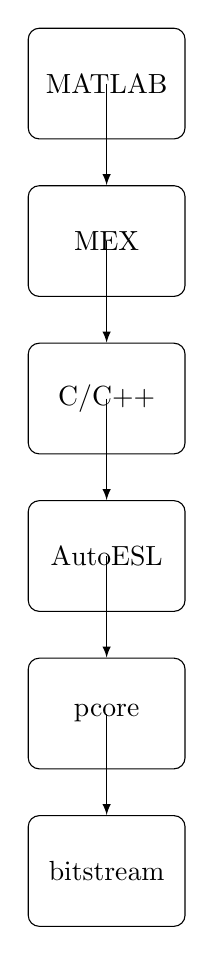
\begin{tikzpicture}[
        block/.style = {
            rectangle,
            draw,
            text width = 5em,
            text centered,
            rounded corners,
            minimum height = 4em},
        arrow/.style = {
            draw,
            ->,
            -latex},
        node distance = 2cm]
    % Place nodes
    \node [block]                   (matlab)    {\progLang{MATLAB}};
    \node [block, below of=matlab]  (mex)       {\progLang{MEX}};
    \node [block, below of=mex]     (cpp)       {\progLang{C/C++}};
    \node [block, below of=cpp]     (autoesl)   {\software{AutoESL}};
    \node [block, below of=autoesl] (pcore)     {pcore};
    \node [block, below of=pcore]   (bitstream) {bitstream};

    % Edges
    \path [arrow] (matlab)  -| (mex);
    \path [arrow] (mex)     -| (cpp);
    \path [arrow] (cpp)     -| (autoesl);
    \path [arrow] (autoesl) -| (pcore);
    \path [arrow] (pcore)   -| (bitstream);
\end{tikzpicture}
    \caption{Design flow for this Thesis}
    \label{thesis:designFlow}
\end{figure}

%%%%%%%%%%%%%%%%%%%%%%%%%%%%%%%%%%%%%%%%%%%%%%%%%%%%%%%%%%%%%%%%%%%%%%%%%%%%%%%%
% Data Sets Used For Testing, Profiling and Benchmarking
%%%%%%%%%%%%%%%%%%%%%%%%%%%%%%%%%%%%%%%%%%%%%%%%%%%%%%%%%%%%%%%%%%%%%%%%%%%%%%%%
\subsection{Data Sets Used For Testing, Profiling and Benchmarking}
\label{software:datasets}
A total of 25 data sets were used for testing, profiling and benchmarking the
commute distance using anomaly detection algorithm. These data sets are
described in detail in \autoref{dataSets}.

\begin{table}
    \centering
    \begin{datasets}
        \dataSetBrief{testCD}{640}{2}
        \dataSetBrief{testCDST}{2000}{2}
        \dataSetBrief{testCDST2}{2000}{2}
        \dataSetBrief{testCDST3}{2000}{2}
        \dataSetBrief{testoutrank}{441}{2}
        \dataSetBrief{pendigits}{4601}{58}
        \dataSetBrief{musk}{67557}{43}
        % TODO: ...
    \end{datasets}
    \caption{Brief description of the data sets}
    \label{dataSets:brief}
\end{table}